\documentclass[10pt,twocolumn,letterpaper]{article}

\usepackage{cvpr}
\usepackage{times}
\usepackage{epsfig}
\usepackage{graphicx}
\usepackage{amsmath}
\usepackage{amssymb}
\usepackage{subfigure}
\usepackage{algorithmic}
\usepackage{algorithm}

\newenvironment{tightenumerate}{
\begin{enumerate}
  \setlength{\itemsep}{1pt}
  \setlength{\parskip}{0pt}
  \setlength{\parsep}{0pt}
}{\end{enumerate}
}

% this makes list spacing much better.
\newenvironment{tightitemize}{
\begin{itemize}
  \setlength{\itemsep}{1pt}
  \setlength{\parskip}{0pt}
  \setlength{\parsep}{0pt}
}{\end{itemize}
}

\cvprfinalcopy % *** Uncomment this line for the final submission

\def\cvprPaperID{****} % *** Enter the CVPR Paper ID here
\def\httilde{\mbox{\tt\raisebox{-.5ex}{\symbol{126}}}}

% Pages are numbered in submission mode, and unnumbered in camera-ready
\ifcvprfinal\pagestyle{empty}\fi

\begin{document}

\title{Segmentation Using Attributes}

\author{Aibo Tian\\
%Institution1\\
%Institution1 address\\
{\tt\small atian@cs.utexas.edu}
% For a paper whose authors are all at the same institution,
% omit the following lines up until the closing ``}''.
% Additional authors and addresses can be added with ``\and'',
% just like the second author.
% To save space, use either the email address or home page, not both
\and
John Edwards\\
%Institution2\\
%First line of institution2 address\\
{\tt\small edwardsj@cs.utexas.edu}
}

\maketitle
\thispagestyle{empty}

%-------------------------------------------------------------------------------
% abstract
%-------------------------------------------------------------------------------
\begin{abstract}
Attributes have been shown to be effective in assisting object detection and
classification, and they provide means to also incorporate semantic
information available to and provided by humans.  On another front, the
combination of segmentation and object classification has been shown to
improve both segmentation and classification.  We present a method of incorporating
attributes into segmentation using a hierarchical methodology.
That is, using attributes as features, we discover attributes of regions
at all levels of a hierarchical segmentation, 
incorporate hierarchical confidences in determining a confidence that
a given region is part of a given object, and segment the image using
these confidences.  We also present results from experiments run using
this method.
\end{abstract}

%-------------------------------------------------------------------------------
% introduction
%-------------------------------------------------------------------------------
\section{Introduction}
Very recent work on using attributes as features \cite{farhadi09, lampert09}
has shown that attributes are an effective way of communicating information
about an object in an image.  Attributes are, in essence, semantic high-level
features.  The attributes of an image are learned using low-level features,
and once learned, they can be used in object detection and also in describing
objects in an image that are unknown.

Image segmentation is a very different field of research and has a very different
goal - that of finding very accurate boundaries of objects in an image.

Our work focuses on leveraging attributes to produce accurate segmentations.
The idea is to find image regions with salient attribute distributions.  If
these regions can be combined together to for larger regions with attribute 
distributions matching some object's canonical distribution then one can
declare the combined region an accurate segmentation for that object.

\begin{figure}
\label{fig:truck}
\centering
\subfigure[]{
\label{fig:trucka}
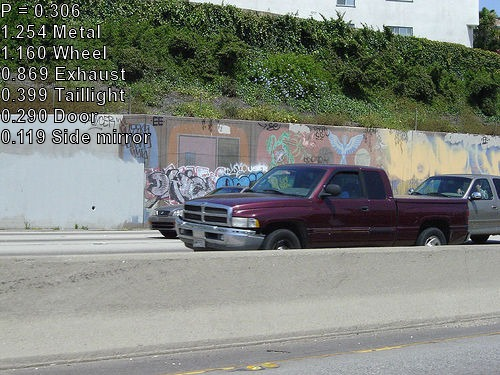
\includegraphics[width=0.22\textwidth]{figures/truck_orig_med.eps}
}
\subfigure[]{
\label{fig:truckb}
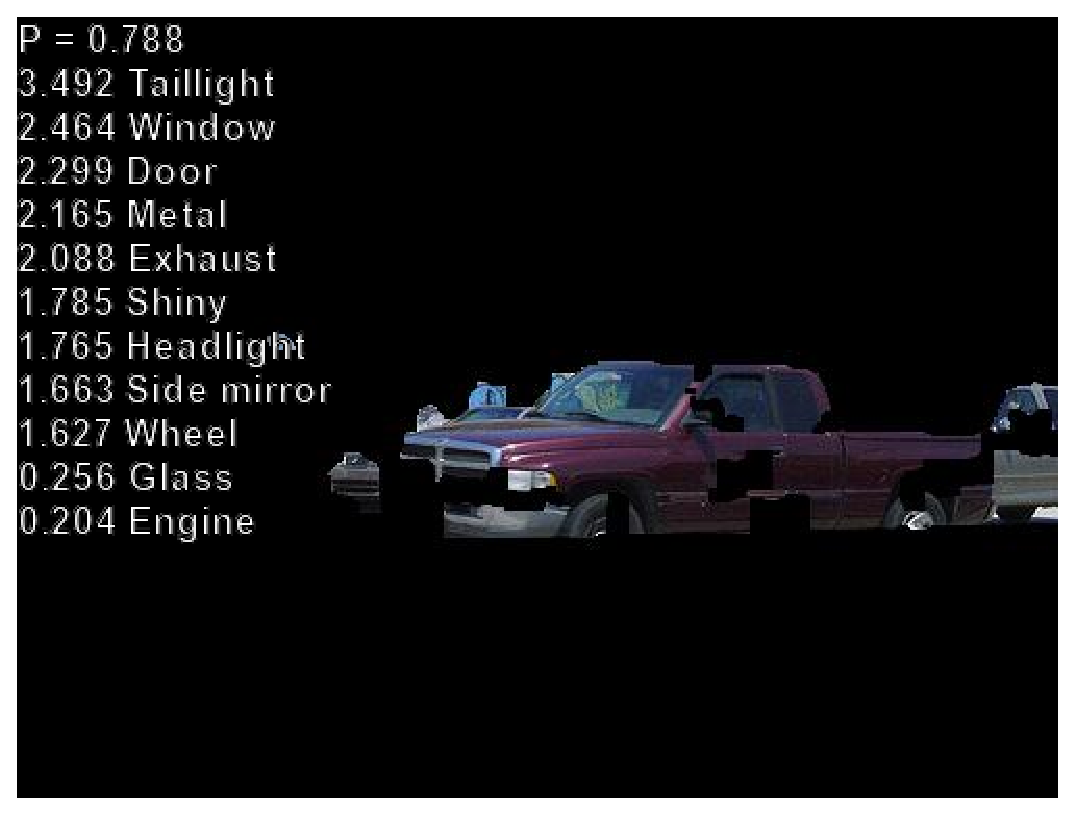
\includegraphics[width=0.22\textwidth]{figures/truck_final_med.eps}
}
\caption{Segmentation by maximizing attribute saliency.  \subref{fig:trucka} shows
the original image with any ``car'' attributes that were predicted.  $P$ is the probability
that the image contains a car.  \subref{fig:truckb} shows the segmented image after
running our segmentation tree pruning algorithm.  As extraneous regions are pruned
more car attributes are predicted and the probability that the remaining image 
contains a car increases.}
\end{figure}

In practice, however, the testing of all combinations of regions to find 
objects is intractable.  We use two approximatory algorithms operating on
a segmentation hierarchy to determine salient regions.  Both are subtractive
algorithms, which first predict attributes on the entire region and then
proceed by observing the effects of removing different regions during
a top-down traversal of the tree.  The benefit of using these methods are
that large regions that clearly don't contribute to attribute saliency
can be pruned from the tree early in the traversal.  This approach avoids
the combinatoric complexity of a full search and, even more, prunes many
regions from the segmentation tree before they even are searched, bringing
the computational complexity, in practice, to roughly $O(n)$ where $n$ is
the number of leaves in the segmentation tree.

While we focus on segmentation of known objects, we anticipate an application
that takes more advantage of attributes: that of segmenting \emph{unknown}
objects from an image that exhibit salient but unrecognized attribute
distributions.  This type of application brings out some of the true power of
attributes, that of assigning semantic meaning to unknown, segmented objects.

This paper is organized as follows: we first discuss related work (\S \ref{sec:related_work})
and then present the algorithm in detail (\S \ref{sec:technical}).  We then discuss results from
a small-scale experiment on images from the pascal 2008 dataset (\S \ref{sec:results}), after which we draw
conclusions and discuss future directions (\S \ref{sec:conclusions}).

%-------------------------------------------------------------------------------
% related work
%-------------------------------------------------------------------------------
\section{Related work}
\label{sec:related_work}
A significant amount of recent work has been done in the area of using
attributes as high-level features for image classification and object
description \cite{farhadi09, lampert09, kumar09}.  
Another area of computer vision, that of segmentation,
has seen a resurgence of popularity as methods to incorporate top-down
information into segmentation have been shown to be highly effective
\cite{borenstein04, pantofaru, gu09, russell06, malisiewicz, leibe04, hoiem05, shotton06}.  
We propose to leverage research done in both of these areas -- attributes
and top-down/bottom-up segmentation -- to produce a combined approach.

Farhadi et al
\cite{farhadi09} use attributes as high-level features for object classification. They
can also describe an image using its attributes alone.
Lampert et al \cite{lampert09}
use the attributes as a intermediate layer between the low-level
features and object classes. Based on this layer, they can predict
disjoint classes that are not seen in the training set.  Both of these
approaches are geared toward object detection and classification.  While
our method goes further, incorporating segmentation, we will be using
the ideas and algorithms in \cite{farhadi09} for assignments of 
attributes to different segmented regions.

Object classification can give some top-down high-level information
for segmentation. On the other hand, segmentation can provide
image-based coherence information for classification. To deal with
the problem that the bottom-up single segmentation is not accurate,
more and more algorithms are based on multiple segmentations. Gu et
al \cite{gu09} uses the hierarchical segmentation algorithm to
generate multiple segments, and detect different parts of objects in
each segment. The final objects are voted for by the various parts.
We will initially be using the same segmentation algorithm used in
this paper, but without discarding the hierarchy.
Russell et al \cite{russell06} detect the whole object in each of
the multiple segment, by assuming that most objects get segmented
correctly at least once during the multiple segmentation. Our approach
will be far less aggressive in that we will use object classes and 
features (attributes in our case) that are known \emph{a priori}.
Pantofaru et
al \cite{pantofaru} use three different segmentation algorithms to
generate the multiple segments. After detecting objects in each
segment, they merge the intersected segments as final results. In
our method, we use common knowledge of distribution of attributes to
merge segments.
Borenstein et al \cite{borenstein04} proposed a method of combining top-down
and bottom-up information to generate a high-quality segmentation.  Their
approach to the top-down is to use exemplar image fragments and match them
to the image and then refining the top-down segmentation using their
segmentation hierarchy.  Our approach is very similar to this in spirit.
While our initial estimate of segmentation is from the bottom-up (while
theirs is from the top-down) we will use the hierarchical information
from the segmentation to boost confidences of segmentation at the lowest
level, similar to what they do.

Another interesting work is that of Gould et al \cite{gould08}.  They use
superpixels for an initial segmentation, build a CRF that includes a
relative location feature in the energy function and minimizes the CRF
for a final segmentation.  The relative location feature is determined
using prior location probability maps.  Our approach is similar to this
as well, in that we will also incorporate relative location information,
although ours will use attributes' relative locations rather than object
classes.  We will also use a CRF for the final segmentation, but will
use a min-cut solution since our labels are binary.
Kumar et al \cite{kumar05} incorporate shape structure into the segmentation by
adding a latent shape parameter to the CRF.  This seems like it would be
a useful addition to our system but make the scope too large.

%-------------------------------------------------------------------------------
% technical approach
%-------------------------------------------------------------------------------
\section{Attribute Detection}
\label{sec:attribute}

Attributes are high-level features which can reflect some semantic properties of objects. Given the attributes, we can do object detection based on the their distribution. We use the same attributes set as \cite{farhadi09}. This set contains three types of attributes, including Shape, Part and Material. All the attributes are listed in figure ?.

We use similar algorithm as \cite{farhadi09} to train the attribute models. Three different type of features are used, such as HOG, texture and color descriptors\cite{farhadi09}. Those features can capture different properties. We use kmeans to quantize all the features. The HOG descriptors are quantized into 1000 clusters, and the texture and color are quantized to 256 and 128 clusters, respectively. All the quantized features are concatenated to form the 1384 deminsional feature. 

For training, we use SVM classifier with Gaussian kernel to train model for each attribute. The precision of all the attributes on the test set is illustrated in figure?.


%Our approach begins with training attribute classifiers.  We trained using
%an SVM with linear kernel.  A set of training images is annotated with objects
%contained in the image, bounding boxes for the objects, and attributes exhibited
%by the image.  We use a subset of the features used in \cite{farhadi09}, namely
%HOG, texture and color descriptors.  The HOG descriptors are quantized into 1000
%kmeans centers, and the texture and color are quantized to 256 and 128 kmeans centers,
%respectively.  Our features differ from \cite{farhadi09} in various ways.  We don't
%use edge descriptors, nor do we generate ``sub-''histograms for 6 cells in the
%image.  The presence of cell histograms would complicate matters when extracting
%features from segmented regions.

\section{Hierarchy Segmentation}
\label{sec:segmentation}

We use the segmentation
approach of \cite{arbelaez09}.  This produces a hierarchical
segmentation by first detecting contours using the \emph{gPb} detector
\cite{maire08}.  Once the contours are detected, regions are discovered using a
watershed algorithm after which an Ultrametric Contour Map (UCM) is constructed,
which defines the region hierarchy. Some example of the hierarchy segmentation is shown in figure?

After the construction of hierarchy segmentation tree, we detect all the attributes in each node, including the intermedia node and leaf node. We use the output of SVM as the confidence (not binary), so each node can be represented by the confidence distribution of all attributes.


\section{Object Detection and Segmentation}
\label{sec:detection}

Our objective is to detect object and segment it out. In our hierarchy segmentation tree, the problem changes to how to select those nodes belong to the desired object. We estimate the probability that a node is belong to object based on the attribute confidence distribution. For each object, we manually give the desired attribute distribution by common knowledge. We use the histogram intersection between the desired distribution and the estimated confidence distribution in each node as the similarity measure. The histogram intersection is calculated as follows:
 
\[ HI(H_{model},H_{pred}) = \frac{|H_{model} \cap H_{pred}|}{|H_{model}|} \]


To select the nodes, we propose two different top-down prune algorithms, additive algorithm and subtractive algorithm. We use the UCM to generate two types of region tree, shown in figure \ref{fig:tree}.
The first tree is an additive tree, where regions are subdivided into successively
smaller regions moving down in the tree.  We call it ``additive'' because the
original image can be reconstructed by adding the regions from each leaf node
together.  The figures show the nodes of the trees as containing images, but in
truth the trees contain binary masks which, when applied to the original image,
produce the shown node contents.

The second tree is ``subtractive.''  The tree has identical structure to the additive
tree and each node contains the inverse of the mask of the corresponding node
in the additive tree.

The final segmentation is obtained by pruning the region tree until a final segmentation
meeting some criterion of absolute or relative attribute saliency is found.
We have two methods for pruning the tree, each showing relative strengths and
weakness.  The first is a semi-greedy additive approach which uses the additive
tree.  The second is a greedy subtractive approach.  We now discuss each of these 
in detail.

\begin{figure*}
\label{fig:tree}
\centering
\subfigure[]{
\label{fig:treea}
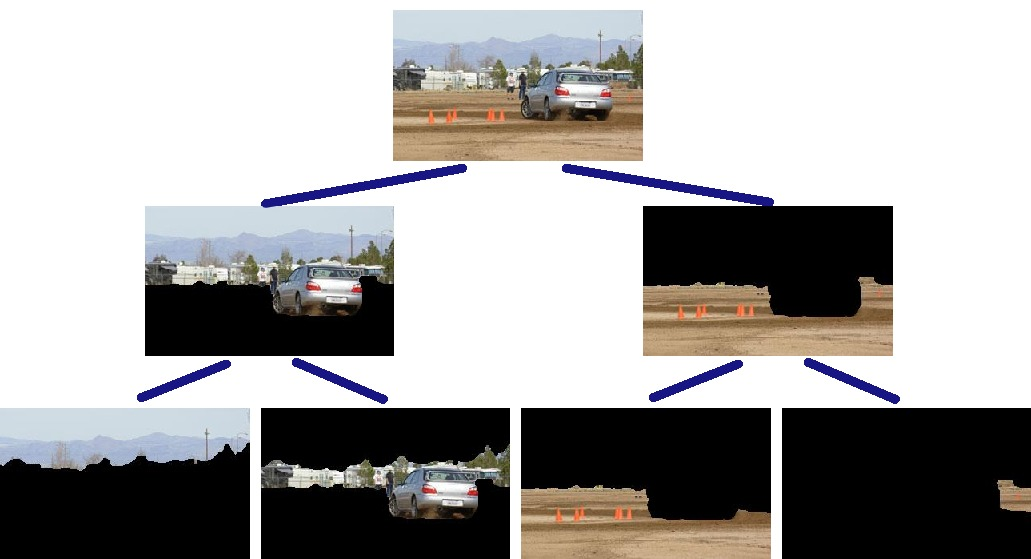
\includegraphics[width=0.45\textwidth]{figures/tree_additive.eps}
}
\subfigure[]{
\label{fig:treeb}
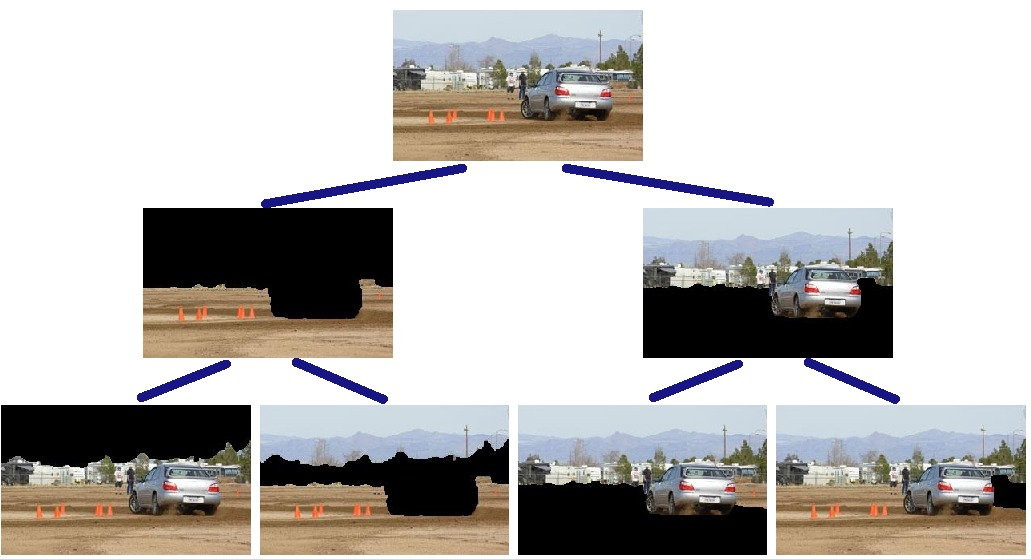
\includegraphics[width=0.45\textwidth]{figures/tree_subtractive.eps}
}
\caption{The two segmentation hierarchies used by the additive \subref{fig:treea}
and subtractive \subref{fig:treeb} algorithms.  The additive hierarchy breaks the
regions into smaller and smaller regions, while the subtractive hierarchy increases
the size of the regions as smaller and smaller chunks are removed from the image.}
\end{figure*}

\subsection{Additive algorithm}
\label{ssec:additive}

This prune algorithm is based on three observations. (1) At least one node in the segmentation tree contrains the whole object. (This is always true since the root node contains the whole image). (2) If both parrent node and child node have high confidence as the object, the segment of child node is more accurate than that of the parrent node. (3) Even if the some node has high confidence as the object, its segmentation still need to improve. The details of the additive algorithm is shown in alg ?.\\

The idea of this algorithm is to find out the minimum discriminative segments, either positive or negative, and combine all of them together to form the final segment. We give three threshold for the similarity measure, $thre\_perf$, $thre\_pos$ and $thre\_neg$ which represent perfect segment, positive segment and negative segment, respectively. If the similarity is above $thre\_perf$, which means the segment is a perfect object, we cut all the nodes below and return this segment. If the similarity is below $thre\_neg$, which means the segment is impossible to be related to the object, we cut all the nodes below too and return NULL. If the similarity is between $thre\_perf$ and $thre\_pos$, which means the node definitely contains the object but the segmentation is not perfect yet, we keep on checking its children nodes to refine the segmentation. The final case is that the similarity is between $thre\_pos$ and $thre\_neg$, which means we are not sure whether there is an object in the node, so we just keep on searching its children. \\

The object detection is based on the output of ADDITIVE\_PRUNE. If the output is not NULL, which means at least one node in the tree has similarity above $thre\_pos$, we think the object is detected in this image.\\ 

(We also plan to do the vertical confidence propogation. But the experiment is too slow, we cannot incorporate it in this draft. We will show it in the final paper.)\\


\begin{algorithm}
\begin{algorithmic}
  \STATE \textbf{input:} 
  \STATE \hspace{3 mm} node $n$ in segmentation tree
  \STATE \hspace{3 mm} desired object model $obj\_model$
  \STATE \hspace{3 mm} threshold for perfect segment $thre\_perf$
  \STATE \hspace{3 mm} threshold for positive segment $thre\_pos$
  \STATE \hspace{3 mm} threshold for negative segment $thre\_neg$
  \STATE \textbf{output:} 
  \STATE \hspace{3 mm} refined segment 
  \STATE
  \STATE $sim=HI(obj\_model,n.conf)$
  \IF{$sim \ge thre\_perf$}
    \STATE return $n.segment$
  \ENDIF
  \IF{$sim \le thre\_neg$}
    \STATE return $NULL$
  \ENDIF
  \STATE $s'=NULL$
  \FOR{$i=1$ to $n.childNum$} 
    \STATE s\{i\}=ADDITIVE\_PRUNE(n.children\{i\},obj\_model,...
    \STATE ... thre\_perf,thre\_pos,thre\_neg)
    \STATE s'=s'+s\{i\}
  \ENDFOR
  \IF{$sim\ge thre\_pos$ and $s'==NULL$}
    \STATE return n.segment
  \ELSE
    \STATE return s'
  \ENDIF
\end{algorithmic}
\caption{ADDITIVE\_PRUNE}
\label{alg:add_prun}
\end{algorithm}
 


\subsection{Subtractive algorithm}

The subtractive algorithm relies on the idea that if removing a region from
an image doesn't significantly affect the probability of the image containing
the object (which probability is obtained using the predicted attribute 
distribution) then that region can be safely removed in the final segmentation.
The algorithm itself is shown in algorithm \ref{alg:sub_prune}.

\begin{algorithm}
\begin{algorithmic}[1]
  \STATE \textbf{input:} 
  \STATE \hspace{3 mm} node $n$ in segmentation tree
  \STATE \hspace{3 mm} master mask $m_m$
  \STATE \hspace{3 mm} probability $P_{root}$ on root node
  \STATE \hspace{3 mm} factor $f$
  \STATE $m_n$ := mask of $n$
  \STATE $H_{pred}$ := predict attributes on image($m_n \cap m_m$)
  \STATE $\displaystyle P_{pred} = \frac{H_{pattern} \cap H_{pred}}{H_{pattern} \cup H_{pred}}$
  \IF{$P_{pred} < f P_{root}$}
    \STATE SUBTRACTIVE\_PRUNE(n.children)
  \ELSE
    \STATE $m_m = m_m \cap m_n$
  \ENDIF
\end{algorithmic}
\caption{SUBTRACTIVE\_PRUNE}
\label{alg:sub_prun}
\end{algorithm}

The subtractive algorithm begins at the root of the tree and predicts attributes.
This attribute distribution and its associated probability $P_{root}$ is assumed to be
canonical for the image.  That is, any final segmentation should not have
significantly less probability $P_{pred}$ than $P_{root}$.  The algorithm traverses
the subtractive tree depth-first, predicting on each node.  
Any node that doesn't have a significant negative effect on the probability
of the presence of the object is removed.  This test is done on line 9.  If the
predicted probability was significantly affected, then we know that the region
must remain.  But it doesn't mean that sub-regions might be able to be pruned
out.  So the procedure is called recursively, checking for smaller regions
that might be able to be pruned (line 10).

If the probability was not significantly affected, then the mask is applied
(line 12) and no recursive call is made.  This is important, because it means
that we can remove large chunks of the image wholesale and bypass predicting
on the node's posterity.

$f$ is an important parameter that requires tuning.  Increasing $f$ makes the
algorithm more conservative, that is, less likely to apply removals.  Decreasing
$f$ makes it more liberal.  We found $f=0.9$ to be a reasonable value for most images.
Figure \ref{fig:f} shows results of adjusting $f$.

The runtime performance of the algorithm is dominated by the prediction step.
Thus the advantage of pruning large chunks early is highly beneficial to 
the runtime of the algorithm.

\begin{figure}
\centering
\subfigure[]{
\label{fig:fa}
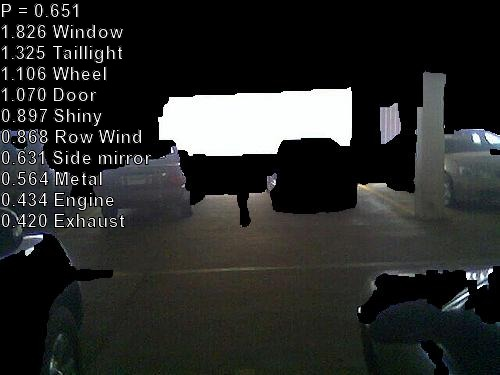
\includegraphics[width=0.22\textwidth]{figures/parking_0.9.eps}
}
\subfigure[]{
\label{fig:fb}
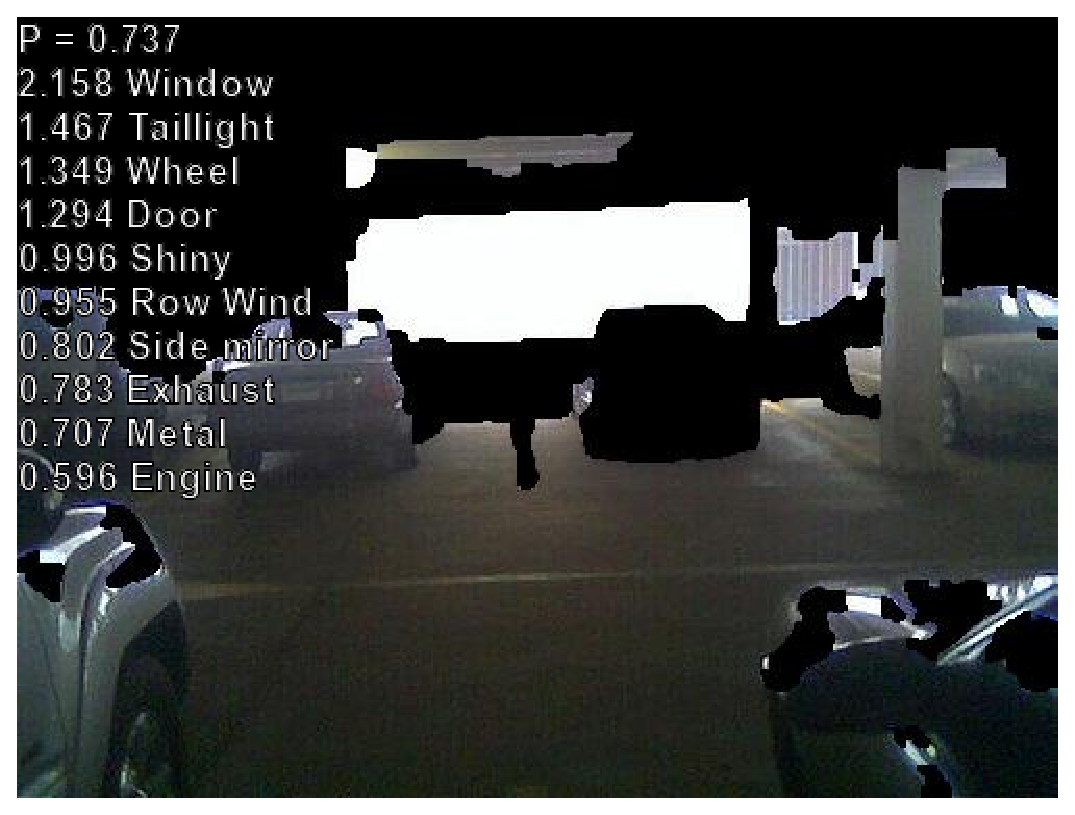
\includegraphics[width=0.22\textwidth]{figures/parking_1.0.eps}
}
\caption{Result of adjusting the factor $f$ in the subtractive algorithm.
\subref{fig:fa} shows running the algorithm with $f=0.9$ and \subref{fig:fb}
shows running the algorithm with $f=1.0$.  Note that \subref{fig:fb} retains
more of the cars, especially the two closest on the right and left, but also
hsa more false-positive pixels, such as the ceiling region of the parking
garage.}
\label{fig:f}
\end{figure}

%-------------------------------------------------------------------------------
% experimental results
%-------------------------------------------------------------------------------
\section{Experimental results}
\label{sec:results}

In this section, we evaluate our attribute based object detection and segmentation algorithm. We will answer four questions. (1) What is the performance of object detection and segmentation? (2) What is the influences of different parameters? (3) What are the advantages of the two pruning algorithms? (4) Is vertical confidence propogation useful? 

\subsection{Dataset}
\label{ssec:dataset}

We use Pascal2008 

Here are some results.
 trained using images from the pascal 
2008 dataset using the same annotations used in \cite{farhadi09}.

%-------------------------------------------------------------------------------
% conclusions and future work
%-------------------------------------------------------------------------------
\section{Conclusions and future work}
\label{sec:conclusions}
Highly dependent on attribute selection and discriminatory ability of attributes.

\subsection*{Acknowledgements}
Thanks to the authors of \cite{arbelaez09} and \cite{farhadi09} for use of their
segmentation and feature extraction code, respectively.

%-------------------------------------------------------------------------------
% bibliography
%-------------------------------------------------------------------------------
{\small
%\bibliographystyle{plain}
\bibliographystyle{ieee}
\bibliography{refs}
}

\end{document}
